\chapter{Conception}

Passer d’une liste de besoins à un système cohérent implique des choix : comment organiser le code, comment modéliser les données, comment éviter qu’un candidat se retrouve dans un état incohérent. Ce chapitre documente les principales décisions de conception derrière JOB4YOU — paquetages, diagramme de classes, scénarios d’interaction et machine à états du cycle de vie d’une candidature.

\section{Introduction}
\label{sec_3_1}
Chaque modèle présenté ici sert directement l’implémentation décrite au chapitre 4 : chaque diagramme correspond à une décision de conception effectivement prise pendant le développement.

\section{Diagramme des paquetages}
\label{sec_3_2}
La figure~\ref{fig_3_1} illustre l’organisation du back-end en paquetages (configuration, sécurité, contrôleurs, services, repositories, entités). L’organisation du front-end et les interactions avec les services externes sont décrites ensuite, puis détaillées aux sections~\ref{sec_3_8} et \ref{sec_3_9}.

% figure 3.1
\setcounter{figure}{0}
\begin{sidewaysfigure}
\centering
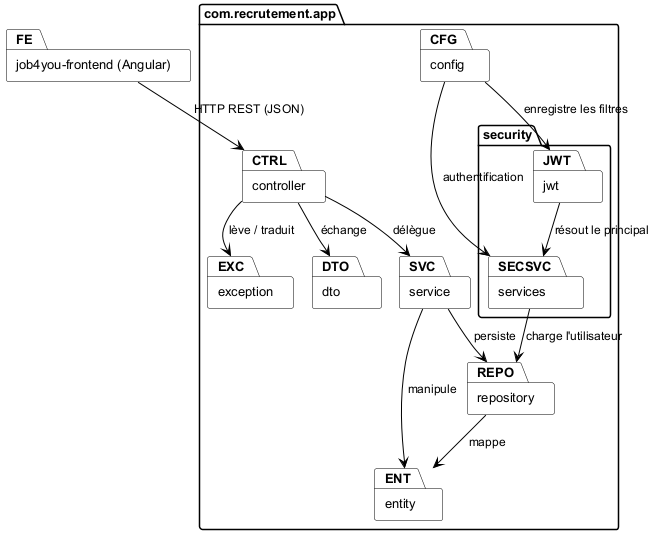
\includegraphics[width=0.98\textheight, height=0.62\textheight, keepaspectratio]{fig3_1}
\caption{Diagramme des paquetages}
\label{fig_3_1}
\end{sidewaysfigure}

Côté back-end, j’ai suivi un découpage classique en couches : la couche controller expose les API REST, la couche service porte la logique métier (règles de gestion, garde-fous, orchestration des appels vers n8n), la couche repository assure la persistance via Spring Data JPA, et les entités JPA modélisent le domaine métier. Côté front-end, chaque page consomme des services Angular dédiés à une ressource métier (candidats, entretiens, feedbacks, offres), qui communiquent eux-mêmes avec le back-end via des appels HTTP authentifiés.

\section{Diagrammes de classes}
\label{sec_3_3}
La figure~\ref{fig_3_2} donne une vue d’ensemble du modèle de données : neuf entités métier principales de la plateforme, leurs attributs caractéristiques et les associations réellement mappées par JPA. Quatorze entités JPA sont persistées au total ; les cinq restantes — notes internes, profils de pondération du scoring, file d’attente n8n, rappels et jetons de réinitialisation — sont des tables d’accompagnement, que l’on retrouve sur le schéma relationnel de la figure~\ref{fig_3_9}. Les deux figures suivantes en proposent des zooms thématiques — le recrutement (figure~\ref{fig_3_2a}), puis les utilisateurs, la sécurité et l’audit (figure~\ref{fig_3_2b}) — afin d’en conserver une lecture confortable.

% figure 3.2
\setcounter{figure}{1}
\begin{figure}[!ht]
\centering
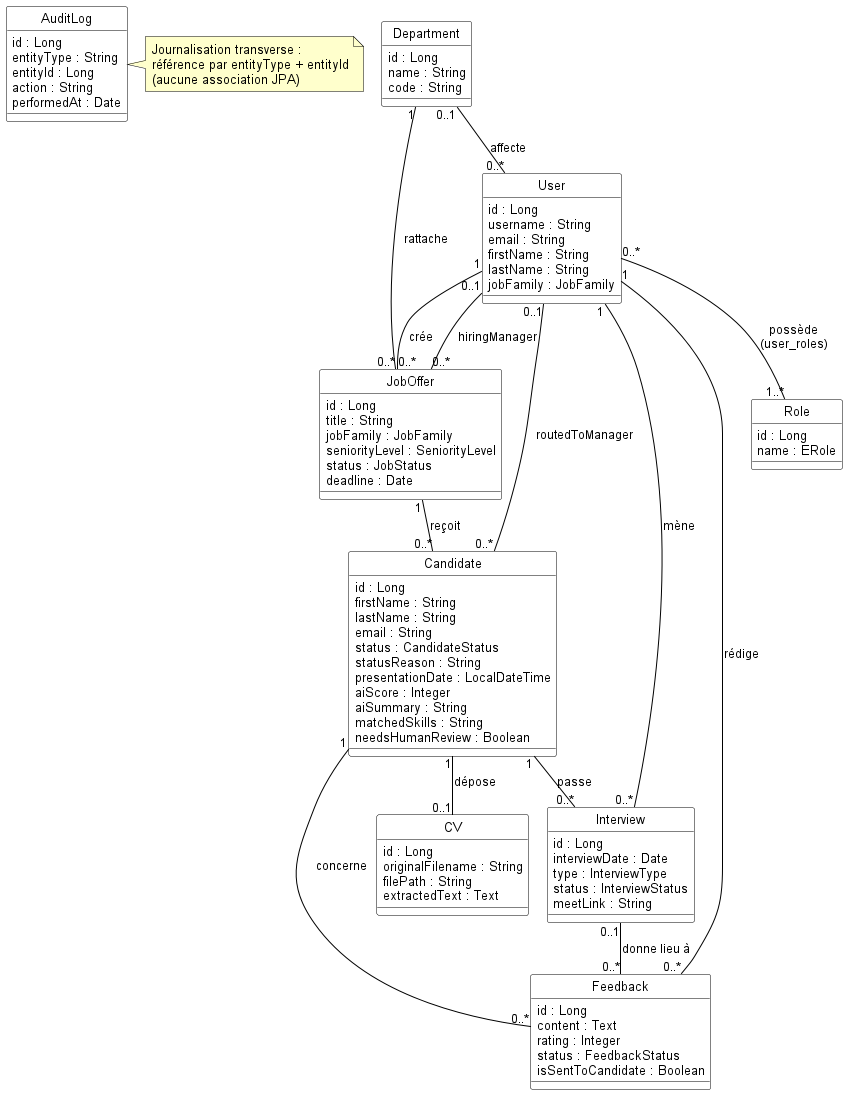
\includegraphics[width=\textwidth, height=0.80\textheight, keepaspectratio]{fig3_2}
\caption{Diagramme de classes — vue globale du domaine métier}
\label{fig_3_2}
\end{figure}

% figure 3.2a
\setcounter{figure}{1}
\begingroup\renewcommand{\thefigure}{3.2a}
\begin{figure}[!ht]
\centering
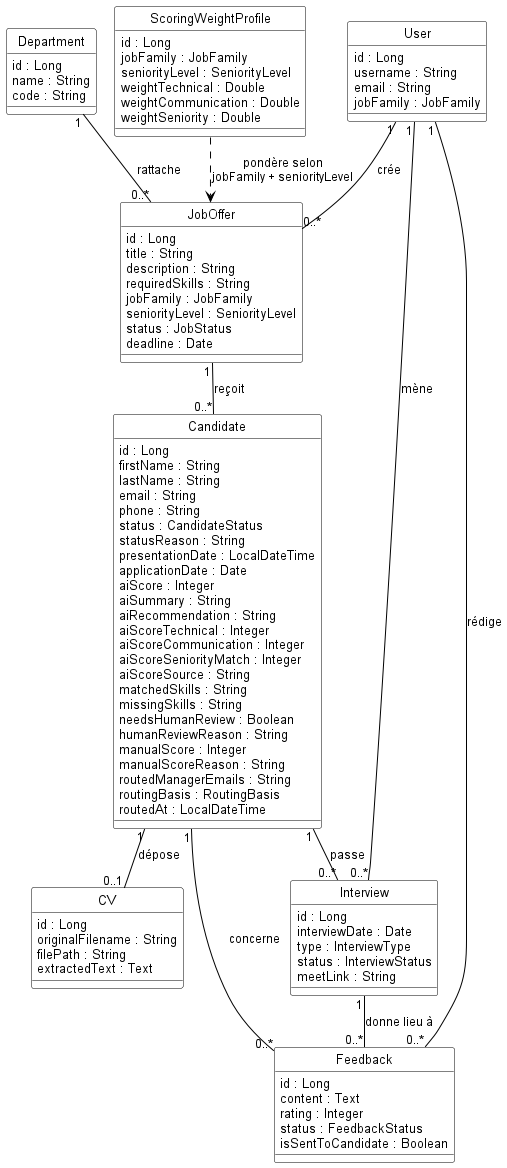
\includegraphics[width=\textwidth, height=0.80\textheight, keepaspectratio]{fig3_2a}
\caption{Diagramme de classes — modèle recrutement}
\label{fig_3_2a}
\end{figure}
\endgroup

Ce modèle fait ressortir plusieurs relations structurantes : un candidat dépose au plus un CV et peut passer par plusieurs entretiens, chacun pouvant donner lieu à un ou plusieurs feedbacks rédigés par un utilisateur (manager ou RH). Une offre d’emploi, rattachée à un département, reçoit plusieurs candidatures. Quant à la classe User, elle centralise l’identité des utilisateurs disposant d’un compte (RH, managers, administrateurs, ainsi que les candidats authentifiés, avec le rôle ROLE\_USER) et porte, via la classe Role, un système de rôles multiples pour une gestion fine des permissions. Les associations de User avec les offres (création), les entretiens (intervieweur) et les feedbacks (auteur) sont matérialisées dans le schéma relationnel (figure~\ref{fig_3_9}) ; le rattachement d’un compte à ses candidatures s’appuie sur l’adresse e-mail du compte, pré-remplie et non modifiable lors du dépôt d’une candidature.

% figure 3.2b
\setcounter{figure}{1}
\begingroup\renewcommand{\thefigure}{3.2b}
\begin{figure}[!ht]
\centering
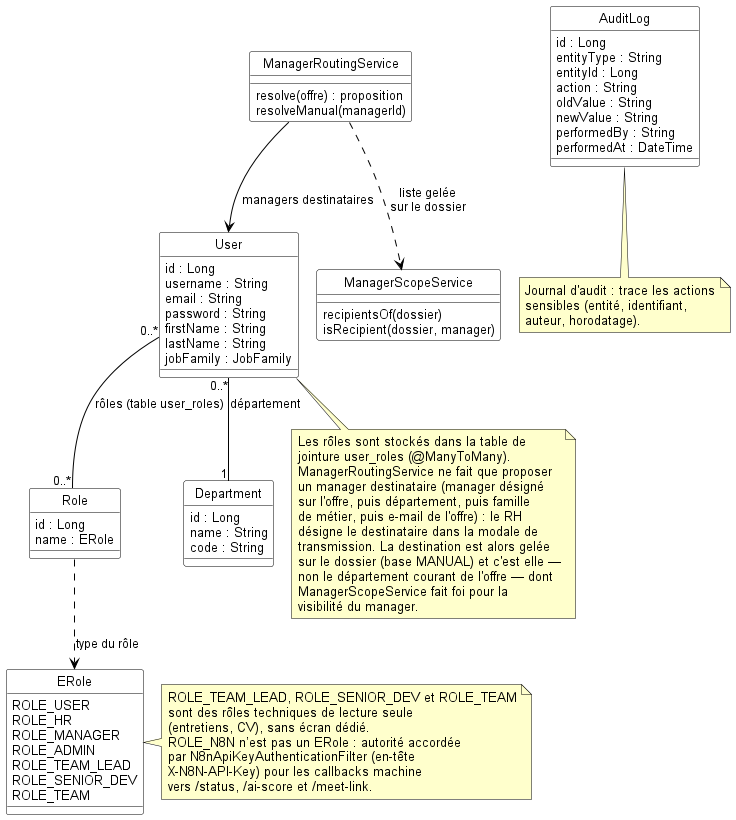
\includegraphics[width=\textwidth, height=0.80\textheight, keepaspectratio]{fig3_2b}
\caption{Diagramme de classes — utilisateurs et sécurité}
\label{fig_3_2b}
\end{figure}
\endgroup

La vue sécurité isole les entités d’authentification et d’audit : chaque utilisateur porte un ou plusieurs rôles (ERole) et, le cas échéant, un rattachement à un département, Manager\-Routing\-Service gèle sur la candidature le manager désigné par le RH, Manager\-Scope\-Service lit cette destination pour borner la visibilité du manager, et AuditLog journalise les actions sensibles.

\section{Séquence technique — Soumission asynchrone et scoring IA}
\label{sec_3_4}
Lors de la soumission d’une candidature, l’application orchestre plusieurs composants internes et externes de manière asynchrone afin de ne pas bloquer l’utilisateur. Comme l’illustre la figure~\ref{fig_3_3}, le front-end Angular transmet la charge utile au back-end Spring Boot, qui persiste immédiatement la candidature (statut APPLIED) ; un mécanisme de file d’attente (outbox) notifie ensuite le serveur d’automatisation n8n, chargé de l’extraction du texte, avant qu’un callback sécurisé ne permette au back-end de solliciter l’API Cohere et d’enregistrer le score de pertinence.

% figure 3.3
\setcounter{figure}{2}
\begin{sidewaysfigure}
\centering
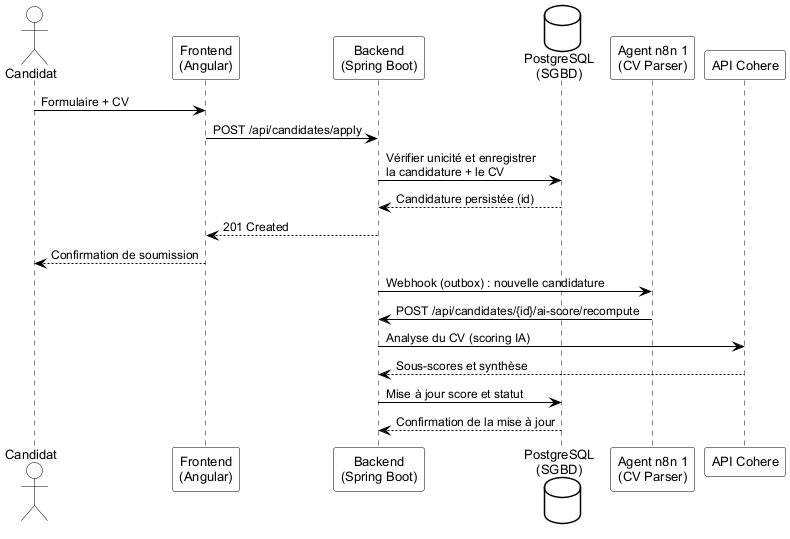
\includegraphics[width=0.98\textheight, height=0.62\textheight, keepaspectratio]{fig3_3}
\caption{Diagramme de séquence technique — Soumission asynchrone et scoring IA}
\label{fig_3_3}
\end{sidewaysfigure}

\section{Diagrammes de séquence objet}
\label{sec_3_5}
Les quatre diagrammes des figures~\ref{fig_3_4}, \ref{fig_3_5}, \ref{fig_3_6} et \ref{fig_3_7} détaillent, au niveau objet, quatre étapes clés du processus de recrutement : la planification d’un entretien, la décision finale de recrutement, l’analyse IA du CV et le routage des managers.

\subsection{Planifier un entretien}
\label{sec_3_5_1}
% figure 3.4
\setcounter{figure}{3}
\begin{sidewaysfigure}
\centering
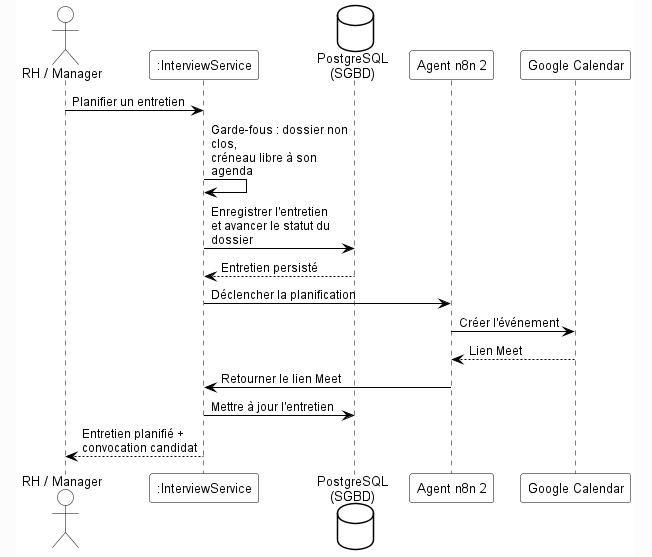
\includegraphics[width=0.98\textheight, height=0.62\textheight, keepaspectratio]{fig3_4}
\caption{Diagramme de séquence objet — Planifier un entretien}
\label{fig_3_4}
\end{sidewaysfigure}

Trois garde-fous ressortent de ce diagramme : la planification écarte un dossier clos (rejeté ou retiré) comme une candidature encore au stade APPLIED dont le CV n’a pas été examiné, et refuse tout créneau chevauchant un entretien déjà réservé du même intervieweur — plusieurs entretiens le même jour restent possibles, jamais au même horaire. Un manager ne planifie enfin que dans son propre agenda, et pour un dossier de son périmètre.

\subsection{Décision finale de recrutement}
\label{sec_3_5_2}
% figure 3.5
\setcounter{figure}{4}
\begin{figure}[!ht]
\centering
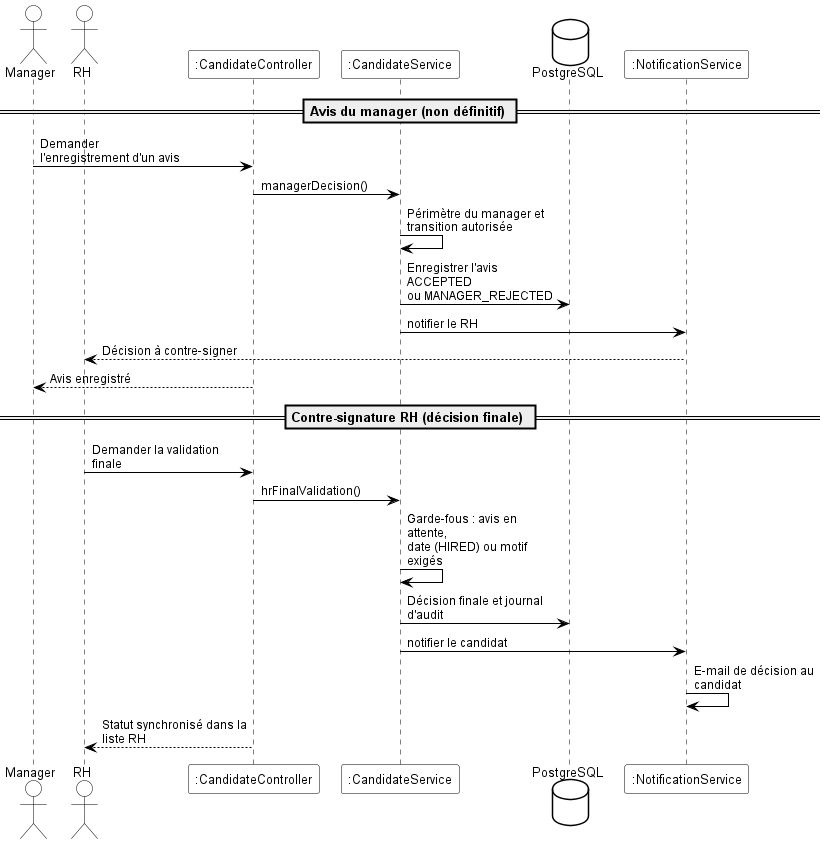
\includegraphics[width=\textwidth, height=0.80\textheight, keepaspectratio]{fig3_5}
\caption{Diagramme de séquence objet — Décision finale de recrutement}
\label{fig_3_5}
\end{figure}

Ce second diagramme illustre le garde-fou central du processus, dont la décision est désormais répartie sur deux niveaux. Le manager consulte le dossier et émet un avis : un refus proposé (MANAGER\_REJECTED), à condition d’être motivé, comme un avis favorable (ACCEPTED), ne sont admis que sur un dossier transmis pour évaluation technique (TECHNICAL\_TEST, INTERVIEW ou FINAL\_INTERVIEW) — les étapes encore côté RH, dont la présélection du CV, ne sont pas instruites par le manager. L’avis est journalisé et notifie le RH par e-mail et dans sa liste de candidats, sans aucun envoi au candidat. Le RH ou l’Administrateur contresigne ensuite via PATCH \path{/api/candidates/\{id\}/final-validation} : HIRED exige la date de présentation des documents et déclenche la convocation, REJECTED exige un motif — enregistré sur le dossier et journalisé, non communiqué au candidat — et déclenche l’e-mail de réponse. Un compte purement manager qui appelle ce point d’entrée, qu’il écrive HIRED ou un statut du pipeline, reçoit une erreur 403. L’ensemble empêche qu’une candidature soit acceptée sans ce premier filtre humain (section~\ref{sec_4_5_8}), et qu’un manager clôture seul le processus.

\subsection{Analyse IA du CV (extraction, scoring via n8n et Cohere)}
\label{sec_3_5_3}
% figure 3.6
\setcounter{figure}{5}
\begin{sidewaysfigure}
\centering
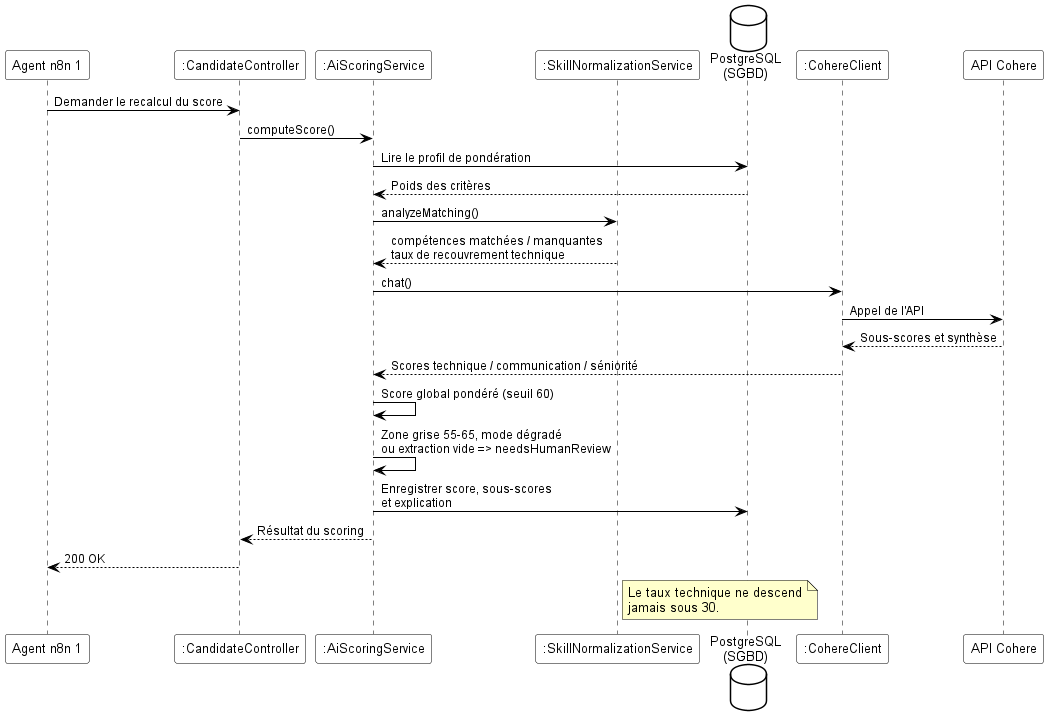
\includegraphics[width=0.98\textheight, height=0.62\textheight, keepaspectratio]{fig3_6}
\caption{Diagramme de séquence objet — Analyse IA du CV}
\label{fig_3_6}
\end{sidewaysfigure}

Ce diagramme détaille, au niveau objet, le cheminement du scoring : le texte du CV est extrait par le back-end au moment même de la soumission, puis la candidature (statut APPLIED) est placée dans la file d’attente interne ; l’agent « CV Parser » n8n est déclenché en arrière-plan et rappelle le back-end via POST \path{/api/candidates/\{id\}/ai-score/recompute}, et c’est le back-end — au travers de son client CohereClient — qui interroge l’API de Cohere, calcule le score et le persiste. Le statut bascule ensuite automatiquement vers CV\_REVIEWED ou AUTO\_REJECTED selon le seuil configuré, sans intervention humaine à ce stade — sauf si le dossier est signalé pour arbitrage, comme le décrit la suite du diagramme. Deux étapes complémentaires figurent sur le diagramme. Avant l’appel au modèle, Skill\-Normalization\-Service harmonise les compétences extraites (k8s devient Kubernetes, postgres devient PostgreSQL) et conserve, après nettoyage, les termes absents du dictionnaire d’alias, afin qu’une compétence rare ne disparaisse pas du comparatif. Après le calcul, le service positionne le drapeau needs\-Human\-Review lorsque le texte extrait est absent ou plus court de cinquante caractères, lorsqu’un écart de séniorité sévère plafonne le score, lorsque celui-ci tombe dans la zone grise comprise entre 55 et 65, ou lorsque l’API de Cohere est indisponible ; dans ce dernier cas le score est marqué SIMULATED et le dossier est dirigé vers un arbitrage humain plutôt que vers une décision automatique (section~\ref{sec_4_4_6}).

\subsection{Passage en évaluation technique — routage et notification des managers}
\label{sec_3_5_4}
% figure 3.7
\setcounter{figure}{6}
\begin{sidewaysfigure}
\centering
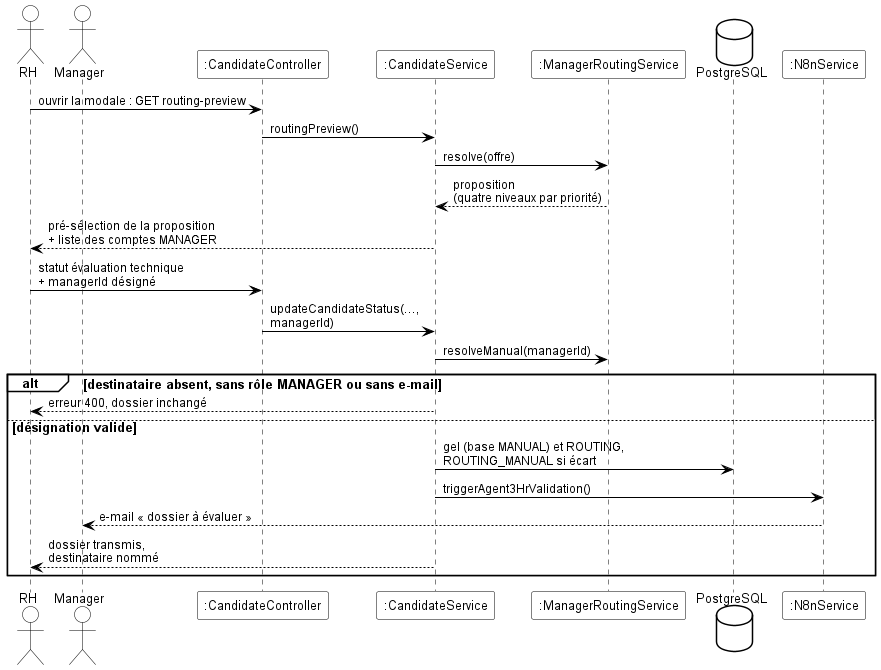
\includegraphics[width=0.98\textheight, height=0.62\textheight, keepaspectratio]{fig3_7}
\caption{Diagramme de séquence objet — Routage et notification des managers}
\label{fig_3_7}
\end{sidewaysfigure}

Ce diagramme détaille la destination et la notification (section~\ref{sec_4_5_5}). La résolution structurelle de Manager\-Routing\-Service — manager désigné sur l’offre, puis département, puis famille de métier, puis ancien champ e-mail — ne produit plus qu’une proposition, pré-sélectionnée dans la modale de transmission : c’est le RH qui désigne le destinataire. Sans désignation, le back-end refuse la transition (erreur 400) et le dossier reste à son statut précédent. Le compte désigné est vérifié — rôle MANAGER, e-mail renseigné — puis gelé sur la candidature avec la base MANUAL ; c’est cette destination, et non le département courant de l’offre, qui borne la visibilité du manager via Manager\-Scope\-Service. Un choix hors proposition reste possible : il est journalisé ROUTING\_MANUAL.

\section{Diagramme d’états — Cycle de vie d’une candidature}
\label{sec_3_6}
Tout au long du processus de recrutement, le statut d’un candidat évolue selon une machine à états précise, représentée à la figure~\ref{fig_3_8}. Le diagramme ne dessine que les transitions les plus représentatives ; les autres transitions autorisées par le garde-fou métier sont détaillées dans le reste de cette section. Cette modélisation garantit la cohérence des transitions et sert de référence pour l’implémentation des contrôles métier côté back-end.

% figure 3.8
\setcounter{figure}{7}
\begin{figure}[!ht]
\centering
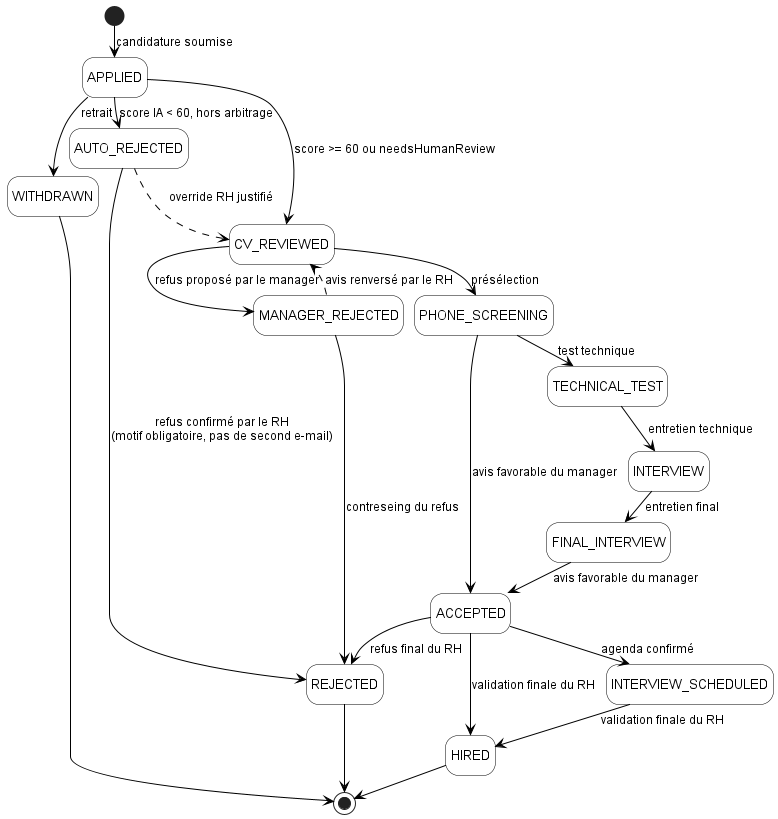
\includegraphics[width=\textwidth, height=0.80\textheight, keepaspectratio]{fig3_8}
\caption{Diagramme d’états du cycle de vie d’une candidature}
\label{fig_3_8}
\end{figure}

Note – le statut INTERVIEW\_SCHEDULED suit ACCEPTED : il matérialise la confirmation de l’agenda et précède l’état HIRED ; il ne désigne pas un entretien d’évaluation, les étapes du pipeline étant closes dès INTERVIEW et FINAL\_INTERVIEW, et rien n’est modélisé pour l’onboarding. Planifier un entretien fait en revanche avancer le dossier à l’étape du type retenu (téléphonique, test, entretien, entretien final) ; une avancée que la machine à états refuse laisse le dossier en place, sans annuler l’entretien.

On y distingue notamment un embranchement automatique piloté par le score de l’analyse IA : le dossier passe en CV\_REVIEWED lorsque le score atteint le seuil de 60/100, en AUTO\_REJECTED lorsqu’il descend sous ce seuil. Les dossiers signalés par le drapeau needs\-Human\-Review — texte de CV inexploitable, écart de séniorité sévère plafonnant le score, zone grise de 55 à 65 ou mode dégradé — font exception à cette règle : ils rejoignent CV\_REVIEWED pour un arbitrage RH et ne sont jamais rejetés automatiquement (section~\ref{sec_4_4_6}). Le statut CV\_REVIEWED y garde un sens unique, le dossier est prêt pour l’examen humain, mais la plateforme ne distingue pas par un état séparé le cas où le score suffit et le cas où un arbitrage est requis : ces deux situations sont signalées par le drapeau et par le motif enregistrés, non par le statut. La décision elle-même est à deux niveaux : ACCEPTED et MANAGER\_REJECTED ne sont que des avis du manager, en attente du contreseing du RH, qui seul atteint HIRED (moyennant la date de présentation des documents) ou REJECTED (moyennant un motif) ; le RH peut aussi prononcer un refus final depuis n’importe quelle étape d’évaluation, et le candidat peut se retirer (WITHDRAWN) tant que le dossier n’est pas clos. Les états véritablement terminaux (HIRED, REJECTED, WITHDRAWN) n’admettent plus aucune modification depuis l’interface d’administration ; AUTO\_REJECTED ne fait plus partie de cette liste et reste entièrement révisable par le RH, qui confirme le refus après examen — REJECTED motivé, sans seconde notification au candidat — ou corrige le score, ce qui réintègre le dossier en CV\_REVIEWED ; la transition vers INTERVIEW\_SCHEDULED, qui suit l’avis favorable, est définie dans la note sous la figure~\ref{fig_3_8}.

Ce rejet automatique n’a rien de définitif, ni d’entièrement hors de contrôle humain : à tout moment, le RH ou l’Administrateur dispose de deux issues. Soit il confirme le refus après examen : le dossier passe alors en REJECTED avec un motif obligatoire, et le candidat ne reçoit pas second e-mail, la notification ayant déjà été émise par l’agent IA. Soit il corrige manuellement le score via un mécanisme de surcharge (manualScore) : la justification y est obligatoire, la correction est journalisée dans l’audit, et le dossier reprend la règle de l’embranchement automatique — une note corrigée à 60 ou plus le réintègre en CV\_REVIEWED et le remet dans le pipeline, une note corrigée sous le seuil le replonge en AUTO\_REJECTED, cette fois sous décision humaine assumée. Le score IA joue ainsi un rôle de filtre de présélection assisté — pas celui d’une autorité décisionnelle autonome.

Le cheminement d’une candidature à travers le scoring IA peut se résumer ainsi : CV candidat $\rightarrow$ dépôt et extraction du texte du CV par le back-end $\rightarrow$ mise en file d’attente et déclenchement asynchrone de l’agent n8n « CV Parser » $\rightarrow$ rappel du back-end via POST \path{/api/candidates/\{id\}/ai-score/recompute} $\rightarrow$ Ai\-Scoring\-Service + CohereClient qui interrogent l’API de Cohere $\rightarrow$ calcul du score global sur 100 $\rightarrow$ orientation automatique vers CV\_REVIEWED (score $\geq$ 60, ou dossier signalé needs\-Human\-Review) ou AUTO\_REJECTED (score < 60 hors zone grise) $\rightarrow$ arbitrage humain possible via le mécanisme de surcharge (manualScore).

Sur le plan de la méthode, le score n’est pas produit par une recherche de similarité vectorielle : la plateforme ne calcule aucun embedding, aucune distance cosinus, et n’exécute aucun modèle entraîné localement. Le back-end appelle le point d’entrée POST \path{/v2/chat} de l’API de Cohere (modèle command-a-03-2025, température nulle, deux cents jetons au plus, sortie contrainte au format JSON) avec un unique message qui fixe le rôle du modèle, impose le schéma de réponse \{technique, communication, séniorité\}, définit ces trois critères et interdit le zéro par défaut : faute d’information exploitable, le modèle doit renvoyer la valeur neutre de 50. Ce message porte les trois champs descriptifs de l’offre (poste, niveau requis, compétences requises) et le texte intégral du CV, lettre de motivation comprise. Les travaux publiés sur l’appariement automatique de CV et d’offres reposent le plus souvent sur une recherche de similarité vectorielle fondée sur des plongements \cite{ref22} ; la solution décrite ici s’en écarte, le score étant produit par un modèle de langage et décomposé en trois critères lisibles plutôt que par une distance entre vecteurs.

La réponse est ensuite relue côté serveur : le bloc JSON est extrait du texte renvoyé, les intitulés de clés sont tolérants aux variantes et une note écrite sous forme de texte numérique (« 86/100 ») est relue comme le nombre 86, avant bornage entre 0 et 100. En revanche, aucune valeur n’est inventée : si l’une des trois clés manque ou n’est pas lisible, l’appel échoue et le mode dégradé local prend le relais, le score étant marqué SIMULATED et signalé pour arbitrage humain (section~\ref{sec_4_4_6}). La valeur neutre de 50 demandée au modèle reste donc une consigne du prompt, non une garantie du serveur : une note absente fait échouer l’appel plutôt que d’être remplacée par un chiffre plus favorable, et un 0 explicitement renvoyé est accepté tel quel. Le score final sur 100 est la moyenne pondérée arrondie (technique $\times$ w1 + communication $\times$ w2 + séniorité $\times$ w3), où les trois poids proviennent du profil de pondération associé à la famille de métier et au niveau de séniorité de l’offre (table scoring\_weight\_profiles, douze profils initialisés, valeurs par défaut 0,5 / 0,2 / 0,3, somme contrôlée à 1 à $\pm$0,01 près). Un CV noté 80 en technique, 70 en communication et 60 en séniorité obtient ainsi 72 avec les poids par défaut, ce que vérifie un test dédié. Les compétences présentées comme correspondantes ou manquantes (matchedSkills / missingSkills), en revanche, ne sont pas revendiquées par le modèle : elles sont calculées localement par le service de normalisation des compétences, à partir d’un dictionnaire d’alias et de recherches à frontière de mot, afin de ne pas reposer sur la seule parole du LLM.

Ce choix de prestataire répond d’abord à une contrainte d’environnement : l’API d’inférence de Hugging Face était bloquée par la politique réseau de l’entreprise, tandis que le point d’entrée de Cohere a été vérifié accessible ; le service est managé, sans dépendance lourde ni poids de modèle à déployer, et sans GPU. La sortie contrainte au format JSON et la température nulle visent à réduire la variabilité des réponses, sans garantir une reproductibilité parfaite tant le modèle et le service externe peuvent évoluer ; la source du score (COHERE ou SIMULATED) est conservée, tandis que la version du modèle, celle du prompt et la réponse brute ne sont pas encore archivées, un enregistrement à prévoir pour rendre une évaluation réellement rejouable, et le classement des offres par compatibilité est regroupé en un seul appel pour un lot d’au plus vingt offres afin de maîtriser le quota. Un modèle embarqué du type sentence-transformers aurait supposé une infrastructure d’exécution et un entraînement adaptés au français des offres ; le besoin réel était une présélection assistée, réversible et expliquée, adossée à un service dont l’indisponibilité est déjà couverte par le mode dégradé local décrit plus haut.

\section{Conception de la base de données}
\label{sec_3_7}
La base de données relationnelle PostgreSQL reflète directement le diagramme de classes présenté en section~\ref{sec_3_3} : chaque entité JPA est mappée sur une table, et les relations One-to-Many et Many-to-One sont matérialisées par des clés étrangères (par exemple job\_offer.hiring\_manager\_id, candidate.routed\_to\_manager\_id, interview.candidate\_id, feedback.interview\_id). J’ai configuré la génération du schéma en mode « update » (Hibernate ddl-auto) — un choix pratique en phase de développement, qui permet de faire évoluer la structure de la base sans perte de données au fil des itérations. En production, ce mode devrait néanmoins céder la place à un outil de migration versionnée comme Flyway ou Liquibase, seul capable de garantir des évolutions de schéma maîtrisées et reproductibles.

Le schéma relationnel de la figure~\ref{fig_3_9} présente l’ensemble des tables générées à partir des entités JPA, avec les clés primaires et étrangères qui matérialisent les relations décrites plus haut.

% figure 3.9
\setcounter{figure}{8}
\begin{sidewaysfigure}
\centering
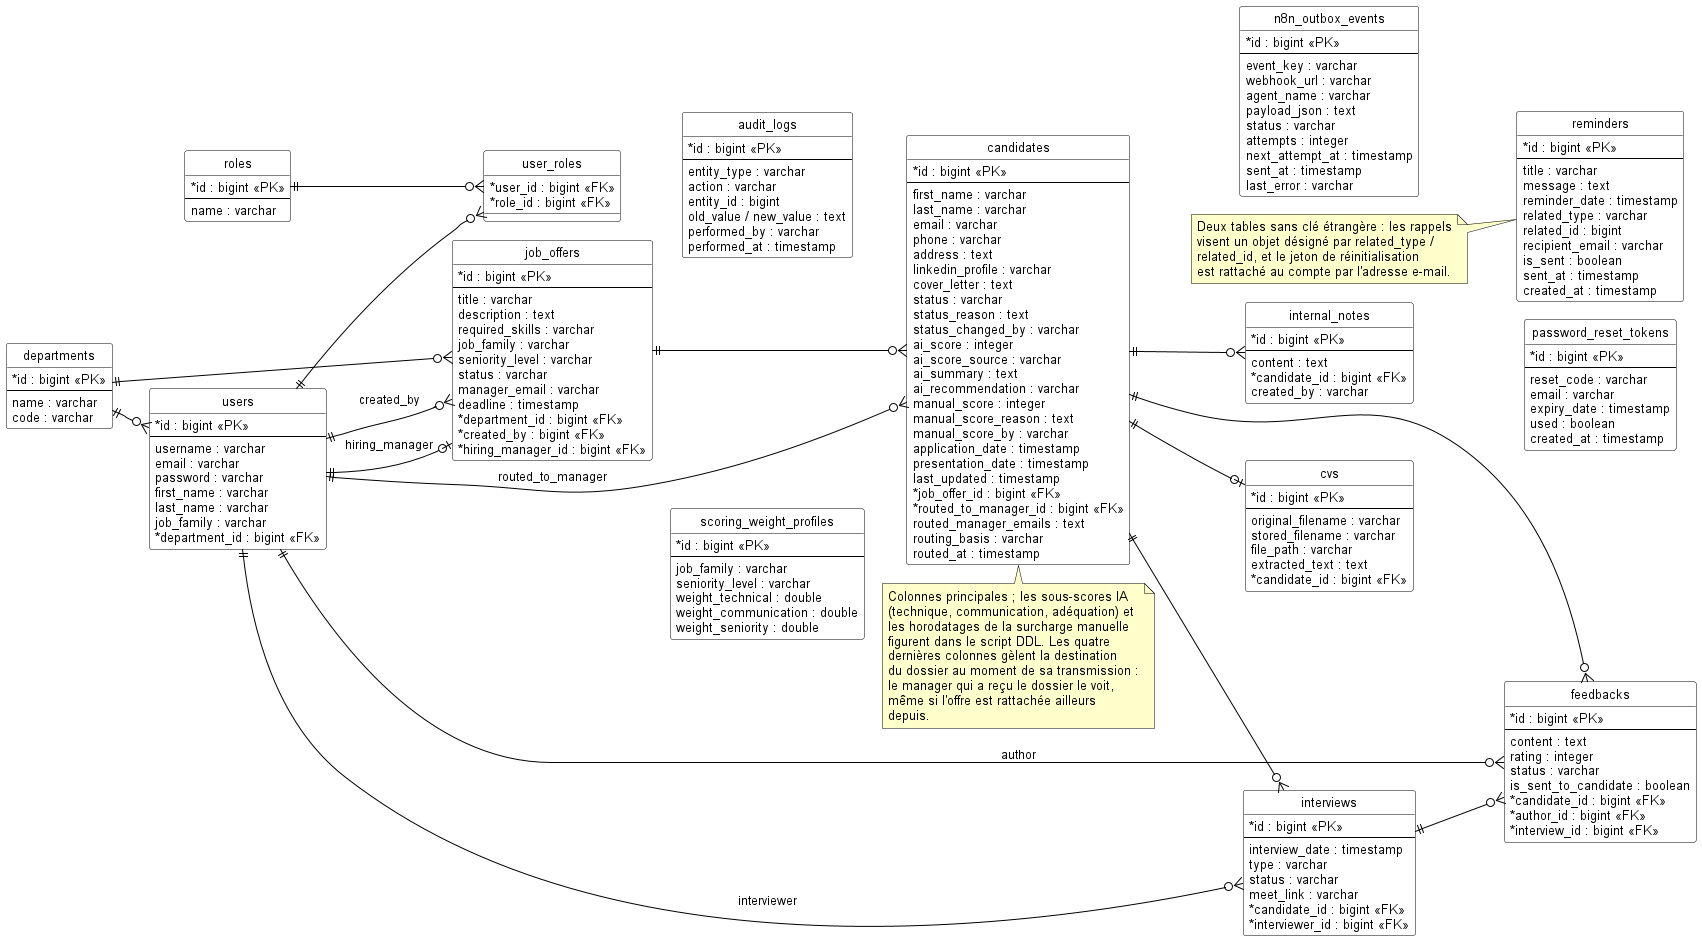
\includegraphics[width=0.98\textheight, height=0.62\textheight, keepaspectratio]{fig3_9}
\caption{Schéma relationnel de la base de données PostgreSQL}
\label{fig_3_9}
\end{sidewaysfigure}

Le schéma relationnel reprend fidèlement les entités JPA : clés primaires préfixées d’un astérisque, clés étrangères suffixées « FK ». On y lit les relations structurantes — département, offres, candidatures, CV, entretiens, feedbacks — et la destination du routage, figée sur le dossier au moment de la transmission (routed\_to\_manager\_id, routed\_manager\_emails, routing\_basis, routed\_at).

\section{Diagramme de composants}
\label{sec_3_8}
Le diagramme de la figure~\ref{fig_3_10} détaille l’organisation de la plateforme en composants logiciels (front-end Angular et back-end Spring Boot), ainsi que leurs dépendances.

% figure 3.10
\setcounter{figure}{9}
\begin{sidewaysfigure}
\centering
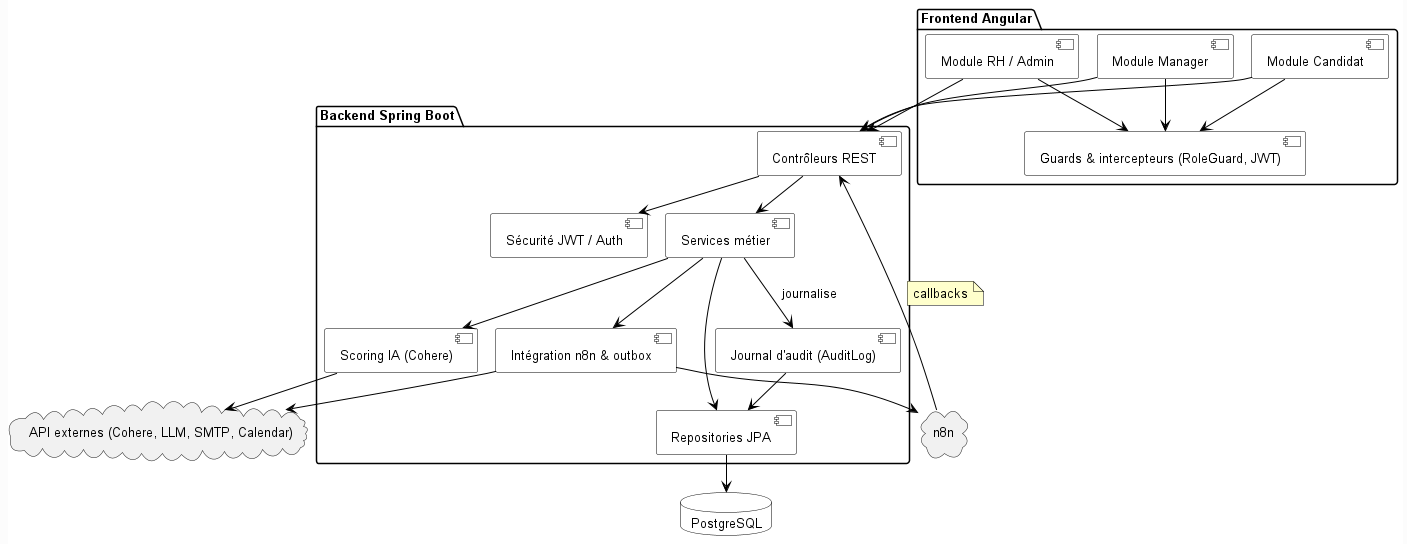
\includegraphics[width=0.98\textheight, height=0.62\textheight, keepaspectratio]{fig3_10}
\caption{Diagramme de composants de la plateforme JOB4YOU}
\label{fig_3_10}
\end{sidewaysfigure}

Chaque service métier (Candidate, Interview, Feedback, JobOffer) s’appuie sur la couche de repositories Spring Data JPA pour la persistance, et sur le service d’audit pour tracer les actions sensibles. Le service Candidate délègue le calcul du score au service de scoring IA, tandis que Candidate et Interview déclenchent chacun les agents n8n compétents via des webhooks.

\section{Diagramme de déploiement}
\label{sec_3_9}
Le diagramme de la figure~\ref{fig_3_11} représente la répartition physique des composants de la plateforme JOB4YOU sur les nœuds d’exécution, ainsi que leurs protocoles de communication.

% figure 3.11
\setcounter{figure}{10}
\begin{sidewaysfigure}
\centering
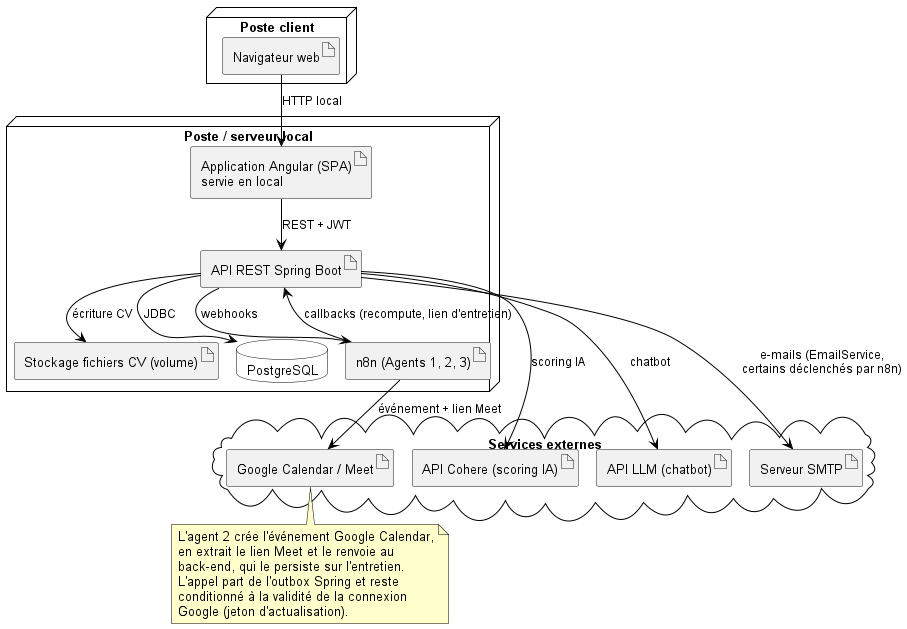
\includegraphics[width=0.98\textheight, height=0.62\textheight, keepaspectratio]{fig3_11}
\caption{Diagramme de déploiement de la plateforme JOB4YOU}
\label{fig_3_11}
\end{sidewaysfigure}

Dans la configuration de développement représentée, le front-end Angular, le back-end Spring Boot, les agents n8n et le stockage des CV s’exécutent sur un même poste local, avec une base de données PostgreSQL (SGBD) pour la persistance. Le front-end communique avec le back-end via des API REST sécurisées par JWT. Le back-end déclenche, via des webhooks HTTP, les agents d’automatisation n8n — lesquels sollicitent à leur tour Google Calendar pour la création réelle de l’événement et du lien Google Meet lors de la planification, et le serveur SMTP pour les notifications — tandis que le back-end appelle lui-même l’API de Cohere pour le scoring IA et l’API OpenRouter pour l’assistant conversationnel.

\section{Conclusion}
\label{sec_3_10}
Ces modèles — paquetages, classes, séquences, états, base de données, déploiement et composants — forment ensemble le plan directeur qui a guidé le développement de l’application, avec les ajustements décrits au chapitre suivant. Reste à voir comment ce plan s’est concrètement traduit en une application fonctionnelle : c’est l’objet du chapitre suivant.
